\chapter{Arrays and Strings}

\textbf{Readings:} CP:AMA 8, 12, 13.

\section{Arrays}

\begin{definition}
An \emph{array} is a data structure containing a fixed number of elements, all of the same type,
stored contiguously (one after another) in memory.
\end{definition}

\begin{lstlisting}[style=c]
int a[6] = {4, 8, 15, 16, 23, 42};
\end{lstlisting}
\begin{center}
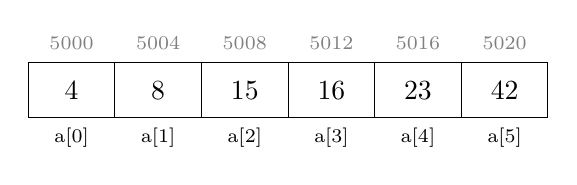
\begin{tikzpicture}[c/.style={draw,minimum width=1.1cm,minimum height=0.7cm}]
  \foreach \v [count=\i from 0] in {4,8,15,16,23,42} {
    \node[c] at (\i*1.1,0) {\v};
    \node[font=\scriptsize] at (\i*1.1,-0.6) {\code{a[\i]}};
    \pgfmathtruncatemacro{\addr}{5000+4*\i}
    \node[font=\scriptsize,gray] at (\i*1.1,0.6) {\addr};
  }
\end{tikzpicture}
\end{center}
Elements are accessed with square brackets: \code{a[0]} is the first element and
\code{a[5]} the last. Array elements are mutable (unless the array is \code{const}):
\code{a[0] = 7;}.

\begin{important}[No bounds checking]
C does \textbf{not} check array indices. \code{a[6]} or \code{a[-1]} silently accesses memory
outside the array: undefined behaviour (corrupting other data, or a segmentation fault).
\end{important}

\subsection{Initialization}

Arrays can only be initialized with braces \code{\{\}}; they cannot be assigned as a whole
after definition (\code{a = b;} is an error).
\begin{lstlisting}[style=c]
int b[5] = {1, 2};          // remaining elements are 0: {1, 2, 0, 0, 0}
int c[5] = {0};             // all zero
int d[] = {1, 2, 3};        // length 3 inferred
int e[5];                   // local: uninitialized (garbage)!
int f[5] = {[2] = 7};       // C99 designated: {0, 0, 7, 0, 0}
\end{lstlisting}

\subsection{Length and size}

The \emph{length} of an array is its number of elements $n$; its \emph{size} is
$n \times \code{sizeof}(\text{element})$ bytes. C does not store the length anywhere. Within the
scope where an array is defined, the length can be computed with
\code{sizeof(a) / sizeof(a[0])}, but this does \emph{not} work once the array is passed to a
function. So we keep track of the length ourselves, often with a constant:
\begin{lstlisting}[style=c]
const int LEN = 6;   // in C99 local arrays may use a variable length
int a[6] = {0};
\end{lstlisting}

\section{Arrays and Pointers}

\begin{important}[An array is (almost) a pointer to its first element]
The value of an array identifier \code{a} is the address of its first element, \code{\&a[0]}.
So \code{a} can be used wherever a pointer to the element type is expected, and
\code{a[i]} is defined to mean \code{*(a + i)}.
\end{important}

\subsection{Passing arrays to functions}

When an array is passed to a function, only the address of the first element is copied (not the
whole array), so the function must also be given the length. The function can mutate the
caller's array; use \code{const} if it should not.
\begin{lstlisting}[style=c]
// sum_array(a, len) produces the sum of the elements of a
// requires: len >= 1
int sum_array(const int a[], int len) {    // same as const int *a
  int sum = 0;
  for (int i = 0; i < len; ++i) {
    sum += a[i];
  }
  return sum;
}

// array_negate(a, len) negates every element of a
// effects: modifies a
void array_negate(int a[], int len) {
  for (int i = 0; i < len; ++i) {
    a[i] = -a[i];
  }
}
\end{lstlisting}

\section{Pointer Arithmetic}

\begin{enumerate}
  \item Adding an integer \code{i} to a pointer \code{p} gives the address of the element
    \code{i} positions later. In ``normal'' arithmetic the address is
    $\code{p} + \code{i} \times \code{sizeof(*p)}$.
  \item Subtracting an integer (\code{p - i}) works in the same way.
  \item Mutable pointers can be incremented and decremented: \code{++p} is \code{p = p + 1}.
  \item You cannot add two pointers.
  \item You can subtract a pointer \code{q} from \code{p} if they have the same type (and point
    into the same array). The result is the number of \emph{elements} between them:
    $(\code{p} - \code{q}) / \code{sizeof(*p)}$ in normal arithmetic. In other words, if
    \code{p == q + i} then \code{p - q == i}.
  \item Pointers of the same type can be compared with \code{<}, \code{<=}, \code{==},
    \code{!=}, \code{>=}, \code{>}.
\end{enumerate}

So \code{a + 1} is \code{\&a[1]}, and \code{*(a + 1)} is \code{a[1]}. Here is the same function
written with pointer arithmetic:
\begin{lstlisting}[style=c]
int sum_array(const int *a, int len) {
  int sum = 0;
  for (const int *p = a; p < a + len; ++p) {
    sum += *p;
  }
  return sum;
}
\end{lstlisting}
Both styles are equivalent; array indexing is usually clearer.

\section{Array ``Map''}

Applying a function to every element of an array is the array equivalent of Racket's
\code{map}. With a function pointer:
\begin{lstlisting}[style=c]
// array_map(f, a, len) replaces each element a[i] with f(a[i])
// effects: modifies a
void array_map(int (*f)(int), int a[], int len) {
  for (int i = 0; i < len; ++i) {
    a[i] = f(a[i]);
  }
}

int a[4] = {1, 2, 3, 4};
array_map(my_sqr, a, 4);   // a is {1, 4, 9, 16}
\end{lstlisting}
Unlike Racket's \code{map}, this mutates the array in place instead of producing a new one.

\section{Sorting}

Sorting is a fundamental problem; here are three classic algorithms (efficiency in Unit~09).
All use the \code{swap} function from Unit~06.

\subsection{Selection sort}

Select the smallest element and swap it into position 0, then the smallest of the rest into
position 1, and so on.
\begin{lstlisting}[style=c]
void selection_sort(int a[], int len) {
  for (int i = 0; i < len - 1; ++i) {
    int pos = i;
    for (int j = i + 1; j < len; ++j) {
      if (a[j] < a[pos]) {
        pos = j;
      }
    }
    swap(&a[i], &a[pos]);
  }
}
// i:   loops from 0 ... len-2; the position to be filled next
// j:   loops from i+1 ... len-1, searching for the next smallest element
// pos: position of the smallest element seen so far
\end{lstlisting}

\subsection{Insertion sort}

Keep a sorted prefix \code{a[0..i-1]}; insert \code{a[i]} into it by swapping it backwards until
it is in place (just like sorting a hand of cards).
\begin{lstlisting}[style=c]
void insertion_sort(int a[], int len) {
  for (int i = 1; i < len; ++i) {
    for (int j = i; j > 0 && a[j - 1] > a[j]; --j) {
      swap(&a[j], &a[j - 1]);
    }
  }
}
\end{lstlisting}
Insertion sort is very fast on arrays that are already (nearly) sorted.

\subsection{Quicksort}

Quicksort (C.\,A.\,R.~Hoare) is a divide-and-conquer algorithm: choose a \emph{pivot}, partition
the array so that smaller elements come before it and larger ones after it, then recursively
sort the two parts. In Racket we built new lists with \code{filter}; in C we partition in place.
\begin{lstlisting}[style=c]
// quick_sort_range(a, first, last) sorts a[first..last] (inclusive)
static void quick_sort_range(int a[], int first, int last) {
  if (last <= first) return;           // 0 or 1 elements
  int pivot = a[first];                // first element as pivot
  int pos = last;                      // where the next "big" element goes
  for (int i = last; i > first; --i) {
    if (a[i] > pivot) {
      swap(&a[pos], &a[i]);
      --pos;
    }
  }
  swap(&a[first], &a[pos]);            // put the pivot in its final place
  quick_sort_range(a, first, pos - 1);
  quick_sort_range(a, pos + 1, last);
}

void quick_sort(int a[], int len) {
  quick_sort_range(a, 0, len - 1);
}
\end{lstlisting}
The C library provides a generic \code{qsort} in \code{<stdlib.h>} (Unit~13).

\section{Binary Search}

Searching an unsorted array for a value requires checking every element (linear search). If the
array is \emph{sorted}, we can compare with the middle element and discard half of the
remaining range each step.
\begin{lstlisting}[style=c]
// find_sorted(item, a, len) produces the index of item in a, or -1
// requires: a is sorted in increasing order
int find_sorted(int item, const int a[], int len) {
  int low = 0;
  int high = len - 1;
  while (low <= high) {
    int mid = low + (high - low) / 2;   // avoids overflow of low + high
    if (a[mid] == item) {
      return mid;
    } else if (a[mid] < item) {
      low = mid + 1;
    } else {
      high = mid - 1;
    }
  }
  return -1;
}
\end{lstlisting}

\section{Multi-dimensional Arrays}

\begin{lstlisting}[style=c]
int m[2][3] = {{1, 2, 3},
               {4, 5, 6}};
m[1][2] = 7;
\end{lstlisting}
C stores multi-dimensional arrays in \emph{row-major order}: \code{m} is laid out as
\code{1 2 3 4 5 6}, so \code{m[r][c]} is at offset \code{r * 3 + c}. When passing a 2D array to
a function, every dimension except the first must be given (\code{int f(int m[][3], int rows)}).
Often it is simpler to use a one-dimensional array and compute \code{a[r * cols + c]} yourself.

\section{Fixed-Length Array Implementation of a Stack}

\begin{lstlisting}[style=c]
#include <assert.h>
#include <stdbool.h>

#define MAXLEN 100

struct stack {
  int len;
  int maxlen;
  int data[MAXLEN];
};

// stack_init(s) initializes *s to an empty stack
void stack_init(struct stack *s) {
  assert(s);
  s->len = 0;
  s->maxlen = MAXLEN;
}

bool stack_is_empty(const struct stack *s) {
  assert(s);
  return s->len == 0;
}

// requires: stack is not empty
int stack_top(const struct stack *s) {
  assert(s);
  assert(s->len > 0);
  return s->data[s->len - 1];
}

// stack_pop(s) removes and produces the top element
// requires: stack is not empty
int stack_pop(struct stack *s) {
  assert(s);
  assert(s->len > 0);
  --s->len;
  return s->data[s->len];
}

// requires: stack is not full
void stack_push(struct stack *s, int item) {
  assert(s);
  assert(s->len < s->maxlen);
  s->data[s->len] = item;
  ++s->len;
}
\end{lstlisting}
All operations are $\bigO(1)$, but the maximum size is fixed when the program is compiled. In
Unit~10 we remove this limitation with dynamic memory.

\section{Strings}

C has no built-in string type. A \emph{string} is an array of \code{char}s terminated by the
\emph{null character} \code{'\textbackslash 0'} (ASCII 0). The terminator is how functions know
where the string ends, so the length does not need to be passed around.
\begin{lstlisting}[style=c]
char a[] = {'c', 'a', 't', '\0'};   // length 4 array, string length 3
char b[] = "cat";                   // the same, more conveniently
char c[10] = "cat";                 // remaining chars are '\0'
\end{lstlisting}
\begin{center}
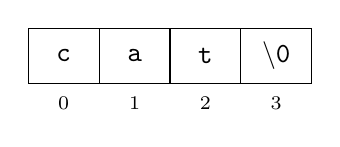
\begin{tikzpicture}[c/.style={draw,minimum width=0.9cm,minimum height=0.7cm}]
  \foreach \v [count=\i from 0] in {c,a,t,\textbackslash 0} {
    \node[c,font=\ttfamily] at (\i*0.9,0) {\v};
    \node[font=\scriptsize] at (\i*0.9,-0.6) {\i};
  }
\end{tikzpicture}
\end{center}

\begin{important}[Null terminator]
An array holding a string of length $n$ needs at least $n+1$ characters. Forgetting room for
\code{'\textbackslash 0'}, or forgetting to add it, leads to functions reading past the end of the
array.
\end{important}

\subsection{String length}
\begin{lstlisting}[style=c]
// my_strlen(s) produces the number of characters in s (excluding '\0')
int my_strlen(const char *s) {
  int len = 0;
  while (s[len] != '\0') {
    ++len;
  }
  return len;
}
\end{lstlisting}

\subsection{String I/O}

The placeholder for strings is \code{\%s}. \code{printf("\%s", s)} prints characters until the
null terminator. \code{scanf("\%s", s)} skips leading whitespace and then reads characters up to
the next whitespace, adding a \code{'\textbackslash 0'}. Note that no \code{\&} is needed: \code{s}
is already a pointer.

\begin{important}[Buffer overflow]
\code{scanf("\%s", name)} with \code{char name[10]} will happily write more than 10 characters if
the user types a long word, overwriting whatever is next in memory. This is a \emph{buffer
overflow}, one of the most common security vulnerabilities. Imagine a bank program where an
account balance is stored right after the name buffer: a long name changes the balance. Always
give a maximum width: \code{scanf("\%9s", name)} reads at most 9 characters (plus the
\code{'\textbackslash 0'}).
\end{important}

\subsection{\code{<string.h>} functions}

\begin{itemize}
  \item \code{strlen(s)}: the length of \code{s} (not counting \code{'\textbackslash 0'}).
  \item \code{strcmp(s1, s2)}: compares lexicographically (by ASCII values). Produces a
    \emph{negative} number if \code{s1} comes before \code{s2}, zero if they are equal, and a
    \emph{positive} number if \code{s1} comes after \code{s2}. (Not necessarily $-1$ and $1$!)
  \item \code{strcpy(dest, src)}: copies \code{src} (including the terminator) into
    \code{dest}. \code{dest} must be large enough.
  \item \code{strcat(dest, src)}: appends \code{src} to the end of \code{dest}. \code{dest} must
    have room for both.
\end{itemize}

\begin{important}[Comparing strings]
\code{s1 == s2} compares the \emph{addresses}, not the contents. Use
\code{strcmp(s1, s2) == 0}.
\end{important}

A possible implementation of \code{strcmp}:
\begin{lstlisting}[style=c]
int my_strcmp(const char *s1, const char *s2) {
  int i = 0;
  while (s1[i] == s2[i] && s1[i] != '\0') {
    ++i;
  }
  return s1[i] - s2[i];
}
\end{lstlisting}

\subsection{String literals}

For each string literal in the program (e.g.\ \code{"hello"} in \code{printf("hello")}), a
null-terminated \code{const char} array is created in the read-only data section. For this reason
the read-only section is also called the \emph{literal pool}. Attempting to modify a string
literal is undefined behaviour (often a segmentation fault).

\section{Arrays vs.\ Pointers}

\begin{lstlisting}[style=c]
char a[] = "pointers are not arrays";
char *p  = "pointers are not arrays";
\end{lstlisting}
\begin{itemize}
  \item \code{a} is an array: 24 bytes on the stack, initialized with a copy of the characters.
    Its contents can be changed (\code{a[0] = 'P';}), but \code{a} itself always refers to the
    same memory (\code{a = ...} is an error). \code{sizeof(a)} is 24.
  \item \code{p} is a pointer variable (8 bytes) pointing at a literal in the read-only section.
    \code{p} can be changed to point somewhere else, but \code{p[0] = 'P'} is undefined
    behaviour. \code{sizeof(p)} is 8. (It would be better declared \code{const char *p}.)
\end{itemize}
So arrays and pointers are closely related (an array ``decays'' to a pointer to its first
element in most expressions) but they are not the same thing.

\section{Summary}
\begin{itemize}
  \item Arrays are fixed-length, contiguous, unchecked; initialize with braces; pass with a
    length.
  \item \code{a[i]} means \code{*(a + i)}; pointer arithmetic counts in elements.
  \item Sorting: selection, insertion, quicksort; binary search on sorted arrays.
  \item 2D arrays are row-major.
  \item Strings are \code{'\textbackslash 0'}-terminated \code{char} arrays; use
    \code{<string.h>}; beware buffer overflow; compare with \code{strcmp}.
  \item String literals live in the read-only literal pool; arrays and pointers differ.
\end{itemize}
